\chapter{Frontend}

Da die Anwendung auf mehreren Plattformen laufen soll wird die Applikation als HTML5 App programmiert.
Dabei besteht das Frontend aus folgenden Views:
\begin{tabularx}{\textwidth}{|l|X|}
    \toprule
    \textbf{ID-Kürzel} & \textbf{Beschreibung} \\
    \midrule
    \endhead
    \hline
    \caption{Einsatzbereiche}
    \label{Einsatzbereiche:tabelle}
    \endfoot
    F-10 & Newsfeed\\
    F-20 & User Login \\
    F-30 & User Registrieren \\
    F-40 & Profilverwaltung und Einstellungen\\
    F-50 & Detailansicht von Einträgen\\
    F-60 & Adminansicht\\
\end{tabularx}

Wie zu sehen ist besteht das Frontend aus sehr wenigen \enquote{Views} und der Benutzer muss immer im Newsfeed oder dem Login landen, wenn er die Seite neu lädt. 
Es muss also kein komplexes Routing System implementiert werden, welches Routen in der Url speichern kann.
Allerdings ist es wichtig, dass sich die Anwendung einen \enquote{Globalen Zustand} teilt,
damit sobald sich z.B. etwas in den Einstellungen ändert diese direkt auf den Rest der Anwendung angewandt wird.
Oder sobald der User einen Eintrag in der Detailansicht bearbeitet, soll dieser im Newsfeed geändert werden.

\section{React.js als View der Anwendung}
React.js soll in Kombination mit Flux für das Frontend eingesetzt werden.
React.js wird dazu für die Erstellung der Komponenten oder der Views verwendet und Flux dient als Architektur der Anwendung.

Der Vorteil von React.js ist, dass die Anwendung in einzelne Komponenten unterteilt werden kann.
Dies erleichter die Entwicklung der Anwendung im Team.
\begin{figure}[H]\label{frontend:react-components}
    \centering
    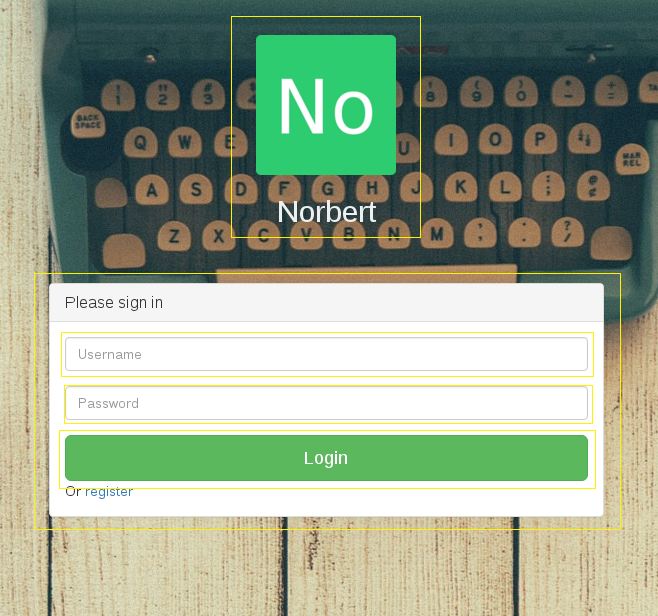
\includegraphics[width=0.4\textwidth]{images/react-components.png}
    \caption{Beispiel Komponenten}
\end{figure}

In dem in Abbildung \ref{frontend:react-components} gezeigten beispiel können alle gelb umramten Teile Komponenten sein.
So kümmert sich die Formular Komponente um das absenden der Request sobald der User versucht sich einzuloggen. 
Andere Komponten wie z.B. Text oder Icons sind lediglich als View gedacht.

\section{Flux als Architekturpattern}
Ein großer Nachteil vieler Kleiner Komponenten in einer Anwendung ist es, dass diese sich einen Zustand könnten, welcher synchronisiert werden muss.
Dazu wird Flux als ein Architektur Pattern eingesetzt.
Die Grundbestandteile dieser Architektur sind Komponenten, Storages, Actions und ein Dispatcher.
Dabei dienen die Komponenten zur Interaktion mit dem User, stellen somit also den \enquote{View} der Anwendung dar.
Die Komponenten können Actions auslösen, welche einfache Funktionen sind die ausgeführt werden.
Diese Actions senden ein Objekt mit einer ID an den Dispatcher, welcher die Objekte an alle Stores verteilt.
Ein Store ist wie der Name schon sagt ein Ort zum lagern von Daten. Jeder Store stellt eine Methode \enquote{handleAction} zur Verfügung.
Diese wird von dem Dispatcher aufgerufen und das Objekt der Action übergeben. 
Anschließend kann der Store aufgrund der in der Action definierten ID seine Daten aktualisieren.
Jetzt können sich Komponenten bei dem Store registrieren um über Änderungen informiert zu werden.
Geschieht dies wird der View der Komponente erneuert. \footnote{Vgl. \url{https://facebook.github.io/flux/}}
\begin{figure}[H]
    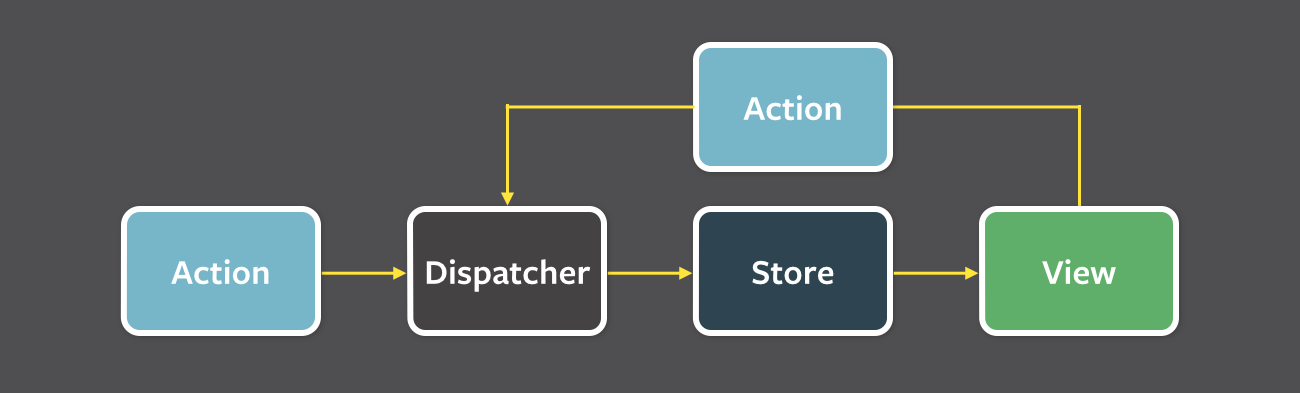
\includegraphics[width=\textwidth]{images/flux.png}
    \caption{Flux}
    \url{https://facebook.github.io/flux/docs/actions-and-the-dispatcher.html#content}
\end{figure}

Diese Architektur unterstütz das Teilen eines Zustandes mehrerer Komponenten, da sich mehrere Komponenten auf einen Storage registrieren 
und Änderungen an dem Zustand der Anwendung immer global über eine Action ausgeführt werden. Somit können alle Stores ihre Daten bei spezifischen Aktionen aktualisieren.
Dadurch wird vermieden, dass sobald sich ein Eintrag ändert eine extra Methode geschrieben werden muss welche den Newsfeed ändert.

